\documentclass[11pt,a4paper]{article}

\usepackage{mathpazo}
\usepackage[bottom=1.5in]{geometry}
\usepackage{fancyhdr}
\usepackage{lastpage} 	
\pagestyle{fancy}		% Declares the page style
\fancyhf{}				% Cleas the header and footer for custumization
\rfoot{Page \thepage\  of \pageref{LastPage}}	% Costumizing the footer
\renewcommand{\footrulewidth}{0.4pt}	% Redifines the width of th the foot-ruler


\usepackage{natbib}			% The bibliography of scientific papers
\bibliographystyle{unsrtnat}% Defines the style of natbib

\usepackage{wrapfig}		% Allows wrapfigures
\usepackage{graphicx}		% Managing of graphics in the document
\usepackage[font=small]{caption}
\usepackage{subcaption}		% Allows captions in subfigures
\usepackage{epstopdf}		% Convertes .eps-files to .pdf-files (figures ex.)
\usepackage{float}			% Allows overrueling of default placing of objects
\usepackage{color}			% Allows colloring of text, pages, ect.
\usepackage{multirow}		% Allows rows to merge

\usepackage[T1]{fontenc}	% Fonts to use for printing characters
\usepackage[utf8]{inputenc} % Allows the user to input accented characters directly from the keyboard
\usepackage[english]{babel} %  Declares languish
\usepackage{amsmath,amssymb,amsthm}	
\usepackage{bm}			% Allows bold and itallic math
\usepackage{mathtools}	% A series of packages enhancing the apperiance of math structures
\usepackage{dsfont}		% Allows double stroke fonts (like sym for real numbers)

\usepackage{titling}
\newcommand{\subtitle}[1]{%
  \posttitle{%
    \par\end{center}
    \begin{center}\large#1\end{center}
    \vskip0.5em}%
}


\setlength{\headheight}{15pt} 


\begin{document}
\author{Alexander S. Madsen}
\title{Introduction to the Error Function}
\maketitle

\section{Introduction}
The following is a brief introduction to the error function $erf(x)$. The article is based the corresponding Wikipedia article about the subject. Furthermore it is written by me and the content contained within it should subsequently be read with a healthy degree of skepticismsm.

\section{The Error Function}
The error function is a non-elementary function defined by the integral
\begin{figure}[b!]
	\centering
	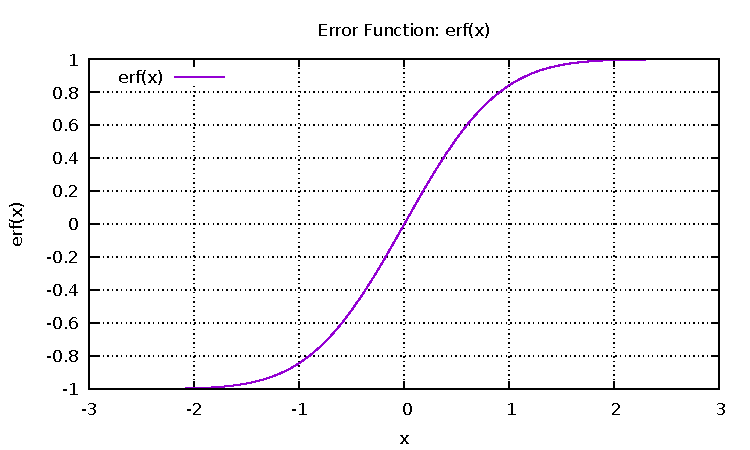
\includegraphics[]{figure.pdf}
	\caption{Plot of the error function in the interval $[-3,3]$ made with gnuplot.}
	\label{fig:erf}
\end{figure}
\begin{equation}
	\textup{erf}(x) = \frac{1}{\sqrt{\pi}} \int_{-x}^{x} \exp{(-t^2)}\ \textup{d}t\ .
\end{equation}
As seen on \ref{fig:erf} it as a characteristic sigmoid shape (s-curve). The error function was developed by the English mathematician and astronomer J. W. L. Glaisher in 1871 in connection with "the theory of Probability, and notably the theory of Errors. It is thus closely related to the normal, or Gaussian, distribution and is predominately used in probability theory. More precisely, for positive values of $x>0$ the error function describes the probability of the error being within the interval $[-x,x]$ for a normally distrusted variable $X$ with expectation value $0$. That is
\begin{equation}
\textup{erf} \left(\frac{a}{\sigma \sqrt{2}}\right)
\end{equation}


\end{document}
